\documentclass[10pt,a4paper]{article}
\usepackage[utf8]{inputenc}

% \usepackage{ngerman}  % german documents
\usepackage{graphicx}  % import graphics einbinden
\usepackage{listings}  % support source code listing
\usepackage{amsmath}  % math stuff
\usepackage{amssymb} % 
\usepackage{a4wide} % wide pages
\usepackage{fancyhdr} % nice headers
\usepackage{tikz} %graphs
\usetikzlibrary{arrows}
\lstset{basicstyle=\footnotesize,language=Python,numbers=left, numberstyle=\tiny, stepnumber=5,firstnumber=0, numbersep=5pt} % set up listings
\pagestyle{fancy}             % header
\setlength{\parindent}{0pt}   % no indentation

\usepackage[pdfpagemode=None, colorlinks=true,  % url coloring
           linkcolor=blue, urlcolor=blue, citecolor=blue, plainpages=false, 
           pdfpagelabels,unicode]{hyperref}
           
% change enums style: first level (a), (b), (c)           
\renewcommand{\labelenumi}{(\alph{enumi})}
\renewcommand{\labelenumii}{(\arabic{enumii})}

%lecture name
\newcommand{\lecture}{
	Bioinformatics III
}           

%assignment iteration
\newcommand{\assignment}{
	Fifth Assignment
}

%set up names, matricle number, and email
\newcommand{\authors}{
  \begin{tabular}{rl}
    \href{mailto:s9alfloh@stud.uni-saarland.de}{Alexander Flohr} & (2549738)\\
    \href{mailto:s9ankupi@stud.uni-saarland.de}{Andrea Kupitz} & (2550260)
  \end{tabular}
}

% use to start a new exercise
\newcommand{\exercise}[1]
{
  \stepcounter{subsection}
  \subsection*{Exercise \thesubsection: #1}

}

\begin{document}
\title{\Large \lecture \\ \textbf{\normalsize \assignment}}
\author{\authors}

\setlength \headheight{25pt}
\fancyhead[R]{\begin{tabular}{r}\lecture \\ \assignment \end{tabular}}
\fancyhead[L]{\authors}


\setcounter{section}{5} % modify for later sheets, i.e. 2, 3, ...
%\section{Introduction to Python and some Network Properties} % optional, note that section invocation sets the section counter + 1, so adapt the setcounter command
\maketitle

\exercise{Cliques and Network Evolution}
\begin{enumerate}
\item Listing \ref{ex1-1} shows source code.
\lstinputlisting[tabsize=4, label=ex1-1,caption={Listing of source code}] {CliqueNetwork.py}

\item Listing \ref{ex1-1} shows source code.

\item Listing \ref{ex1-1} shows source code.

\item The number of cliques stays approximately the same independent of the time step because approximately the same amount of edges are added which are removed as shown in figure \ref{fig-1}, table \ref{tab1} and table \ref{tab2}. The amount of cliques of size 3 increases rather than the one of larger cliques because a less edges added may result in a small clique.
\begin{figure}
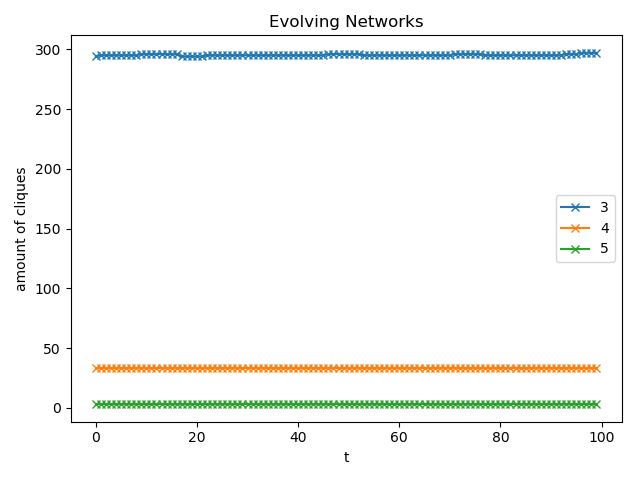
\includegraphics[scale=1]{plotTask1_100.png}
\caption{Number of cliques of size 3, 4 and 5 at the beginning and after each time step as a function of time with t = 100}
\label{fig-1}
\end{figure}

\begin{table}[!h]
\label{tab1}
\begin{tabular}{llll}
clique size & number of cliques before evolution & number of cliques after evolution\\
\hline
3 & 294 & 300\\
4 & 33 & 33\\
5 & 3 & 3\\
\end{tabular}
\caption{Number of cliques of size 3, 4 and 5 at the beginning and after letting it evolve for 100 time steps}
\end{table}

\begin{table}[!h]
\label{tab2}
\begin{tabular}{llll}
clique size & number of cliques before evolution & number of cliques after evolution\\
\hline
3 & 294 & 327\\
4 & 33 & 27\\
5 & 3 & 3\\
\end{tabular}
\caption{Number of cliques of size 3, 4 and 5 at the beginning and after letting it evolve for 1000 time steps}
\end{table}

\item The goal of randomising networks this way is to create random permutations of a network. In this way the behaviour of similar networks may be studied and the networks quality may be rated.\\
Listing \ref{ex1-2} shows source code.
\lstinputlisting[tabsize=4, label=ex1-2,caption={Listing of source code}] {RandomizedNetwork.py}

\item Assuming a p-value of 0.05, none of the clique sizes were significantly enriched, see table \ref{tab3}.\\
Listing \ref{ex1-3} shows source code.
\lstinputlisting[tabsize=4, label=ex1-3,caption={Listing of source code}] {MotifNetwork.py}
\begin{table}[!h]
\label{tab3}
\begin{tabular}{ll}
clique size i & $p_i$\\
\hline
3 & 0.38\\
4 & 0.27\\
5 & 1.0\\
\end{tabular}
\caption{Number of randomised networks in which the
number of cliques is at least as high as in the original network divided by the number of randomised networks for each clique size}
\end{table}
\end{enumerate}

\exercise{Annotations in Protein Protein Interaction Networks}
\begin{enumerate}
\item Implemented in \texttt{PPIGONetwork.py}, see Listing \ref{ex2}

\item Required information provided in table \ref{table:ex2a}
\begin{table}[!h]
\caption{Reults for exercise 5.2 b}
\label{table:ex2a}
\begin{tabular}{l l}
Task & Result\\
\hline
total number of proteins and interactions in the network & 17087\\
total number of unique annotations in the network & 275472\\
total number and percentage of proteins without any annotation & 2334 (13.6595\%)\\
smallest number of annotations per protein & 0\\
average number of annotations per protein & 7.013\\
highest number of annotations per protein & 184\\
smallest number of associated proteins per annotatio & 1\\
average number of associated proteins per annotatio & 10.302\\
highest number of associated proteins per annotatio & 1519\\
\end{tabular}
\end{table}

\item In table \ref{table:ex2c}, we see the five most and least annotated GO terms. We see that the most annotated GO terms are all involved in crucial biological processes for cell viability. In this way, we have important transcription factors, which regulate the different expression levels. Additonally, we have one GO term encoding signal transduction, which is also important for cell communication, appoptosis, etc. Further, the GO terms are relatively unspecific, so they do not describe just one specific process, - this fewer information content leads to a high number of annotations . Therefore it is no surprise that these GO terms are high annotated.\\
In contrast, the least annotated GO terms describe various, precise biological processes. Therefore they can only be assigned to a specific subset of human proteins. Therefore we see only a few annotations of them. So they are less common but have a higher information content than the most annotated proteins GO terms.
\begin{table}[!h]
\caption{Reults for exercise 5.2 b}
\label{table:ex2c}
\begin{tabular}{c c c}
Task & Result\\
\hline
\multicolumn{3}{c}{Most Common}\\
\hline
GO term & Occurrence & Biological Process\\
\hline
GO:0006351 & 1519 &  transcription, DNA-templated\\
GO:0045944 & 1001 &  positive regulation of transcription by RNA polymerase II\\
GO:0007165 & 980 & signal transduction\\
GO:0006357 & 937 &  regulation of transcription by RNA polymerase II\\
GO:0006355 & 740 & regulation of transcription, DNA-templated\\
\hline
\multicolumn{3}{c}{Least Common}\\
\hline
GO term & Occurrence & Biological Process\\
\hline
GO:0000003 & 1 &  reproduction \\
GO:0000011 & 1 & vacuole inheritance\\
GO:0000032 & 1 & cell wall mannoprotein biosynthetic process\\
GO:0000053 & 1 &  argininosuccinate metabolic process \\
GO:0000097 & 1 & sulfur amino acid biosynthetic process\\
\end{tabular}
\end{table}
\item Not implemented

\item Not implemented

\item Listing \ref{ex2} shows source code.
\lstinputlisting[tabsize=4, label=ex2,caption={Listing of source code}] {PPIGONetwork.py}

Program output for human network with time measurement:\\
\texttt{Start program\\
1. Create Network\\
2. Initialize Mapping\\
3. Assign Alternative Names\\
4. Assign Go terms\\
Initialization completed\\
--------------------- Overview ---------------------\\
Total number of proteins:			17087\\
Total number of protein interactions:		275472\\
Number of proteines without GO annotation:	2334 (13.6595072277\%)\\
Smallest number of GO annotations per protein	0\\
Average number of GO annotations per protein	7.01293380933\\
Highest number of GO annotations per protein	184\\
Smallest number of proteins per GO annotations	1\\
Average number of proteins per GO annotations	10.3017537827\\
Highest number of proteins per GO annotations	1519\\
5 most annotated GO terms:	[('GO:0006355', 740), ('GO:0006357', 937), ('GO:0007165', 980), ('GO:0045944', 1001), ('GO:0006351', 1519)]\\
5 fewest annotated GO terms:	[('GO:0000003', 1), ('GO:0000011', 1), ('GO:0000032', 1), ('GO:0000053', 1), ('GO:0000097', 1)]\\
\\
real	5m56,373s\\
user	5m53,229s\\
sys	0m0,304s\\
}

\end{enumerate}
\end{document}